\documentclass[a4paper, 12pt]{article}
\usepackage{graphicx}
\usepackage{caption}
\usepackage{wrapfig}
\usepackage{float}
\usepackage{cmap}
\usepackage{tikz}
\usepackage{enumitem}
\usepackage{multirow}
\usepackage[utf8]{inputenc}
\usepackage{array,graphicx,caption}
\usepackage[english, russian]{babel}
\usepackage{amsmath, amsfonts, amssymb, amsthm, mathtools}

\title{Формула Ричардсона-Дэшмана}
\date{}

%-----------------------------------СOLONTITLE-------------------------------------------

\usepackage{fancyhdr}

   \pagestyle{fancy}
   \fancyhead{Формула Ричардсона-Дэшмана}
   \fancyhead[L]{}
   \fancyhead[R]{Грошев Максим}
   \fancyfoot[C]{\thepage}

%------------------------------------------------------------------------------------------
\usepackage{extsizes}
\begin{document}

%-----------------------------------TITLEPAGE-----------------------------------------------

    \begin{titlepage}
    \maketitle
    \thispagestyle{empty}

            \begin{figure*}[h]
            \centering
            
\includegraphics[scale=1.3]{./pics/rt.png}
            \end{figure*}

             \vspace{15em}
             \begin{flushright}
                 \normalsize Выполнил:\\
                             Грошев М.А. Б01-207б
             \end{flushright}

             \begin{center}
                    \vfill \normalsize Долгопрудный 2025
             \end{center}
    \end{titlepage}

%-------------------------------------------------------------------------------------------

\newpage
\setcounter{page}{1}

\textbf{Цель работы:}  На практике убедиться в выполнении зависимости описываемой формулой
Ричардсона-Дэшмана. Убедиться в выполении закона "$\frac{3}{2}$"\\

\par
\textbf{Используемое оборудование:} 2 источника постоянного напряжения на 300 В, 3 мультиметра,
, микроамперметр, вакуумный диод, пирометр \\

%--------------------------------------------THEORY------------------------------------------

\section{Теоретические сведения}


\newpage

%-------------------------------------------------------------------------------------------

\section{Экспериментальнaя установкa и методика эксперимента}

\begin{figure}[H]
        \centering
        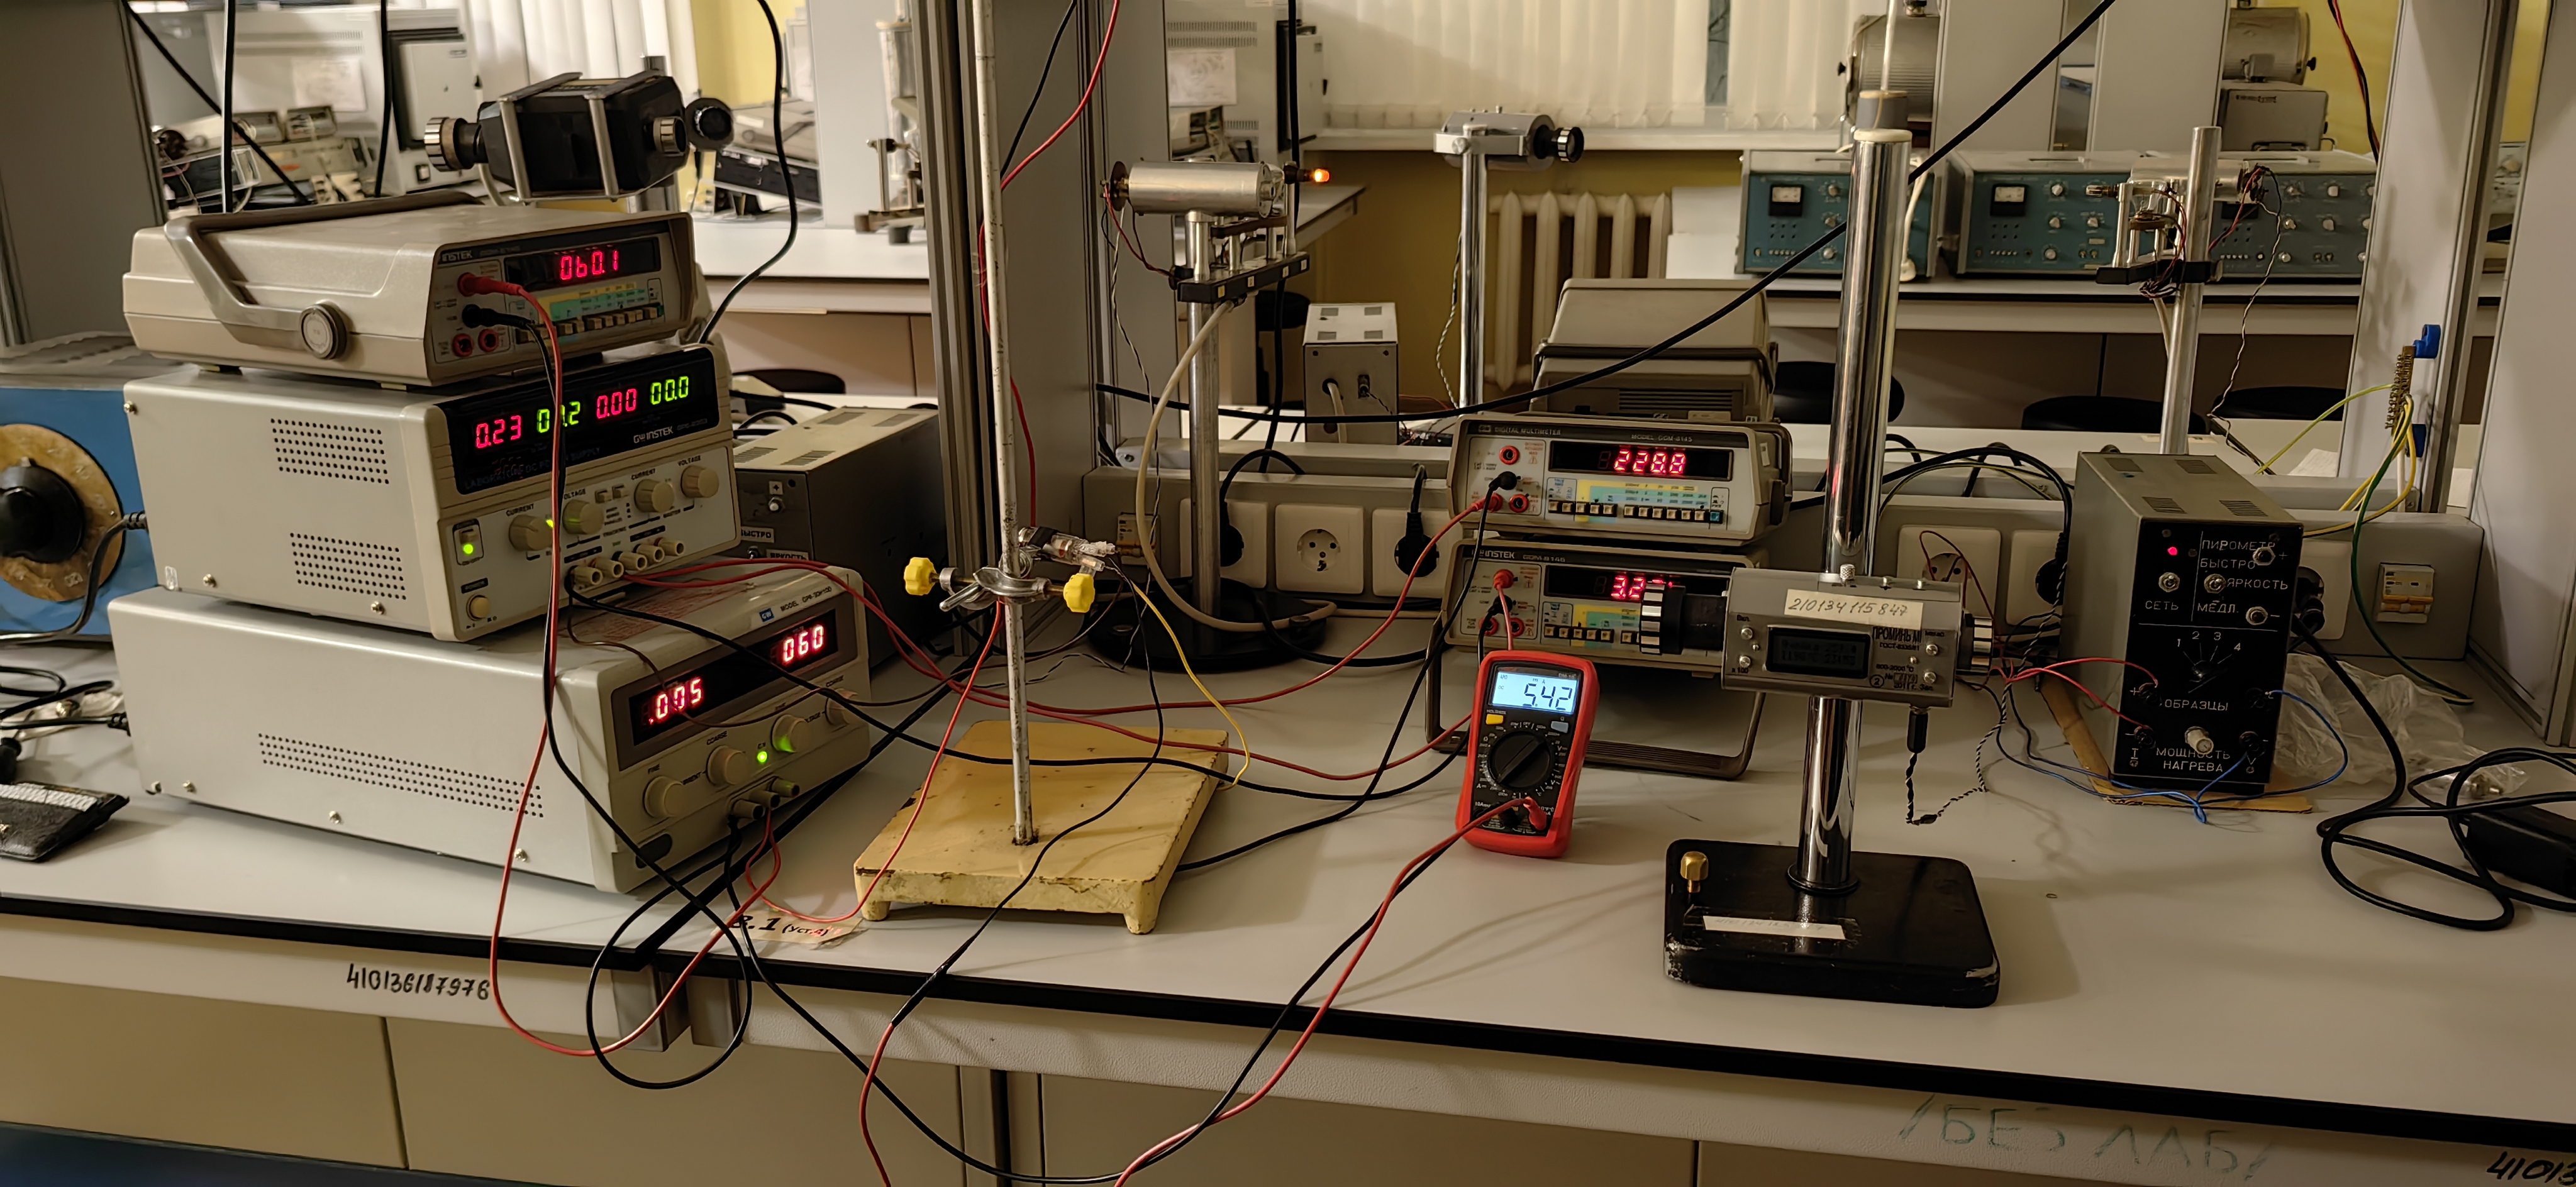
\includegraphics[scale=0.08]{./pics/setup_ph.jpg}
        \\
        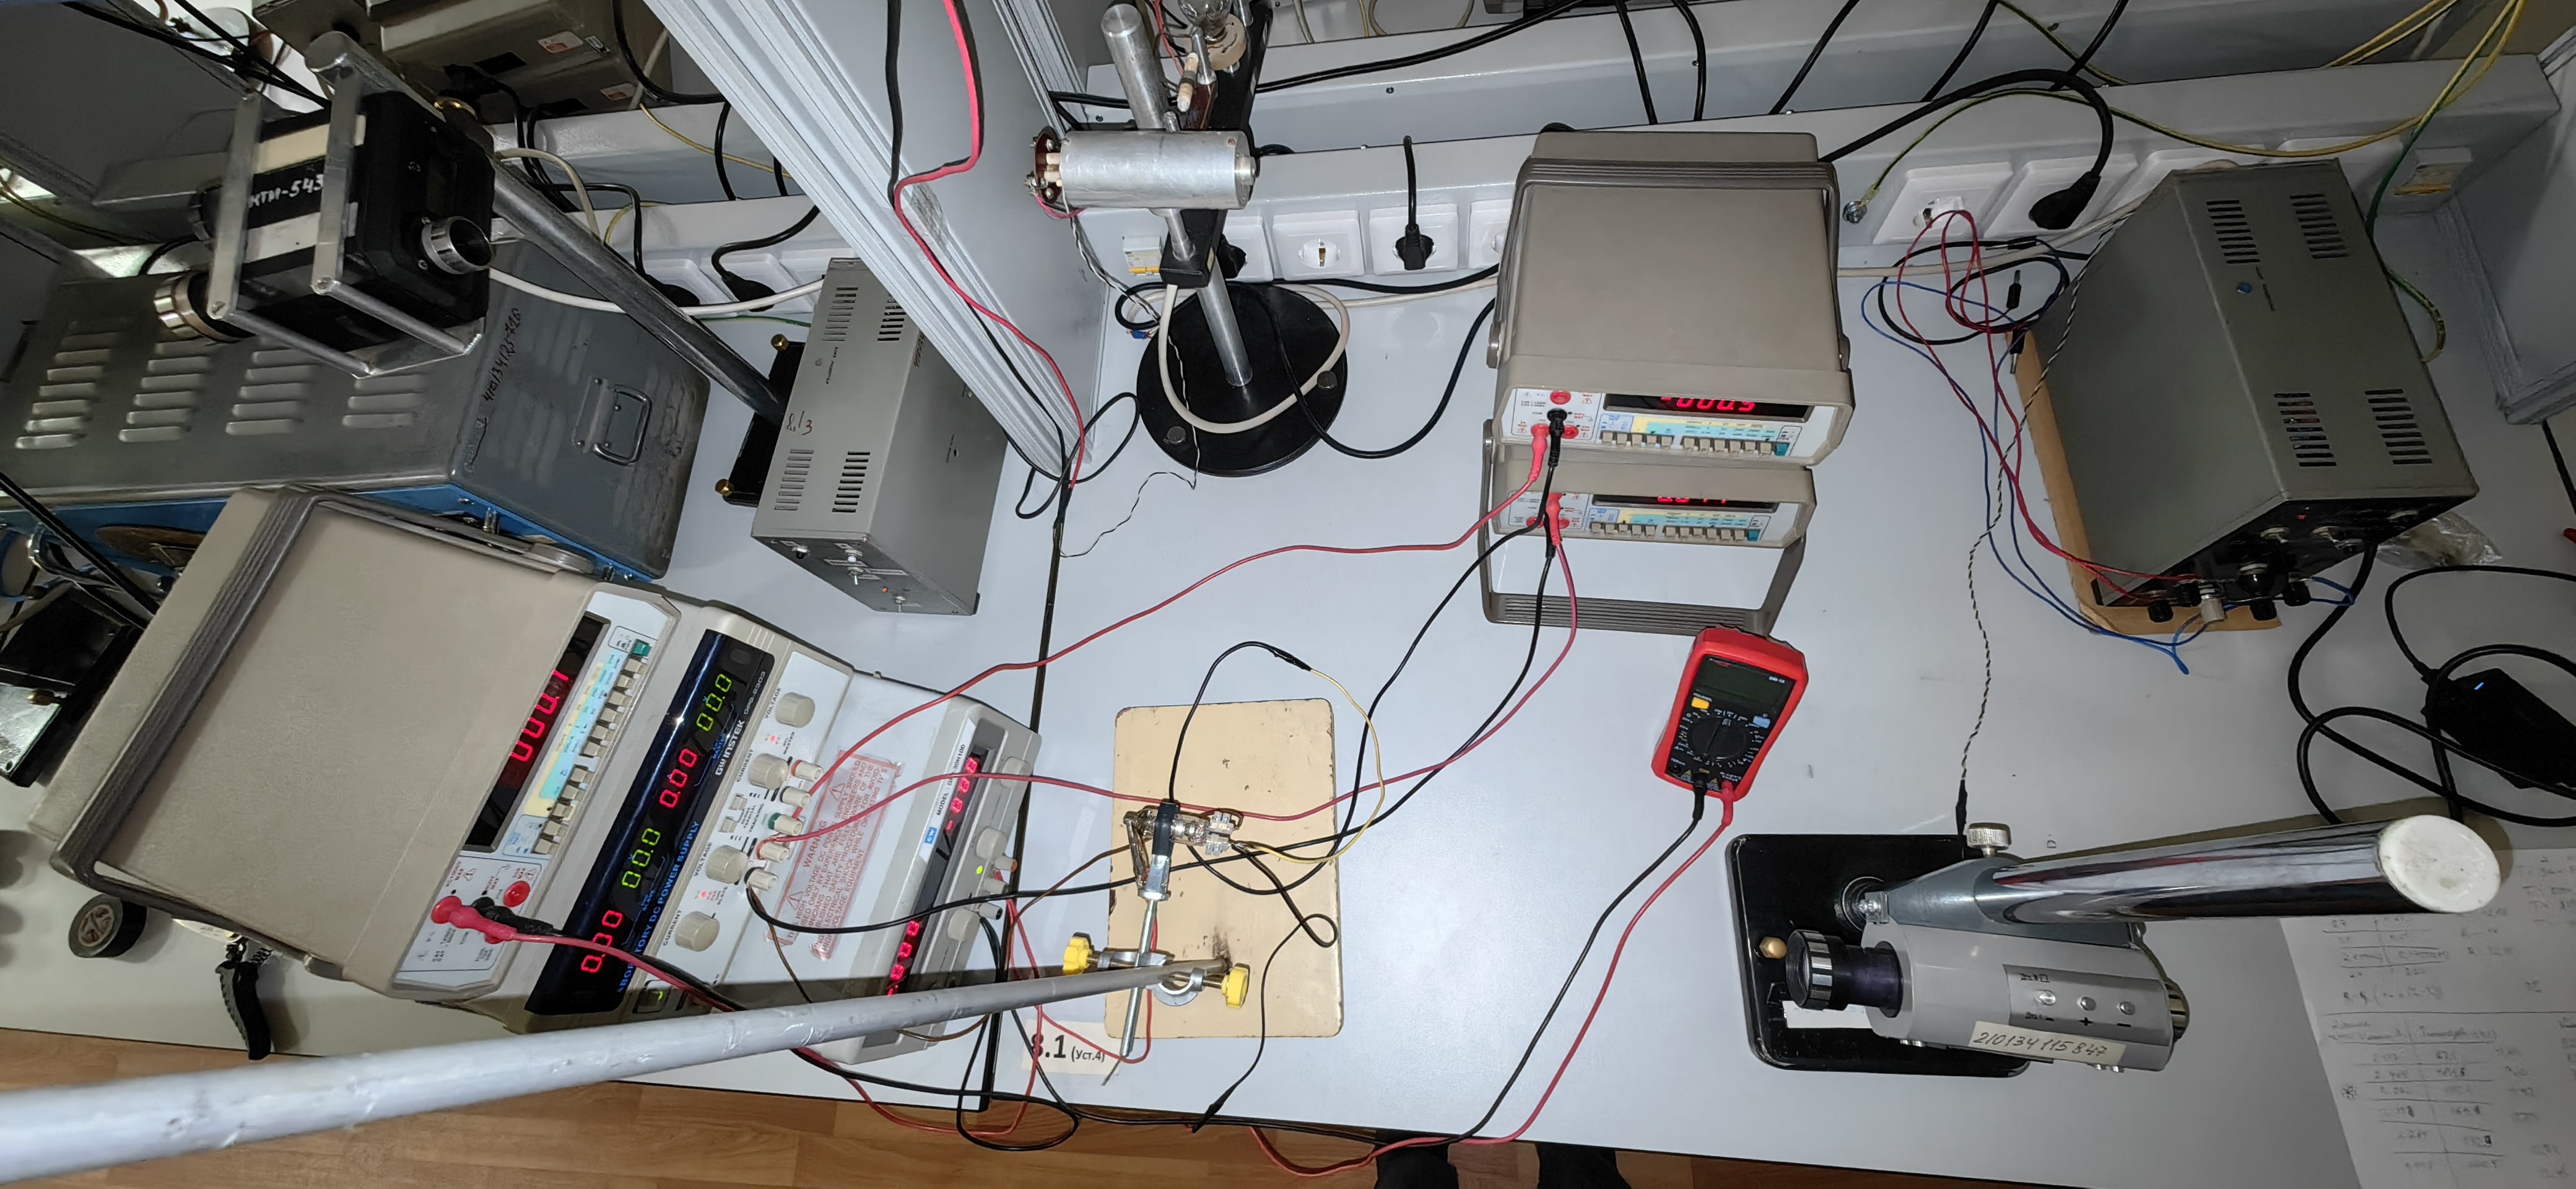
\includegraphics[scale=0.08]{./pics/setup_ph_up.jpg}
        \caption{Фото экспериментального стенда}
        \label{ris:setup_ph}
\end{figure}

\begin{figure}[H]
        \centering
        
\includegraphics[scale=0.3]{./pics/setup_sh.jpg}
        \caption{Блок-схема экспериментального стенда}
        \label{ris:setup_sh}
\end{figure}



\begin{tabular}{m{0.45\linewidth}m{0.6\linewidth}}
На рис ($\ref{ris:setup_ph}$, $\ref{ris:setup_sh}$) Изображена эксперемнтальная установка. При помощи
одного из генереторов выставлялось постоянное напряжение$(2 - 3 \text{В}$) на катоде(номер ножки).
При нагревании нить-катод начинала светиться красным цветом и мы определяли температуру катода.
\par
Далее с использованием второго генератора выставлялось положительная разность потенциалов между катодом и анодом$(0 - 200 \text{В}$).
Напряжение поднималось до того момента пока мы не выходили на плато на вольтамперной характеристике.
    &
     \centering
     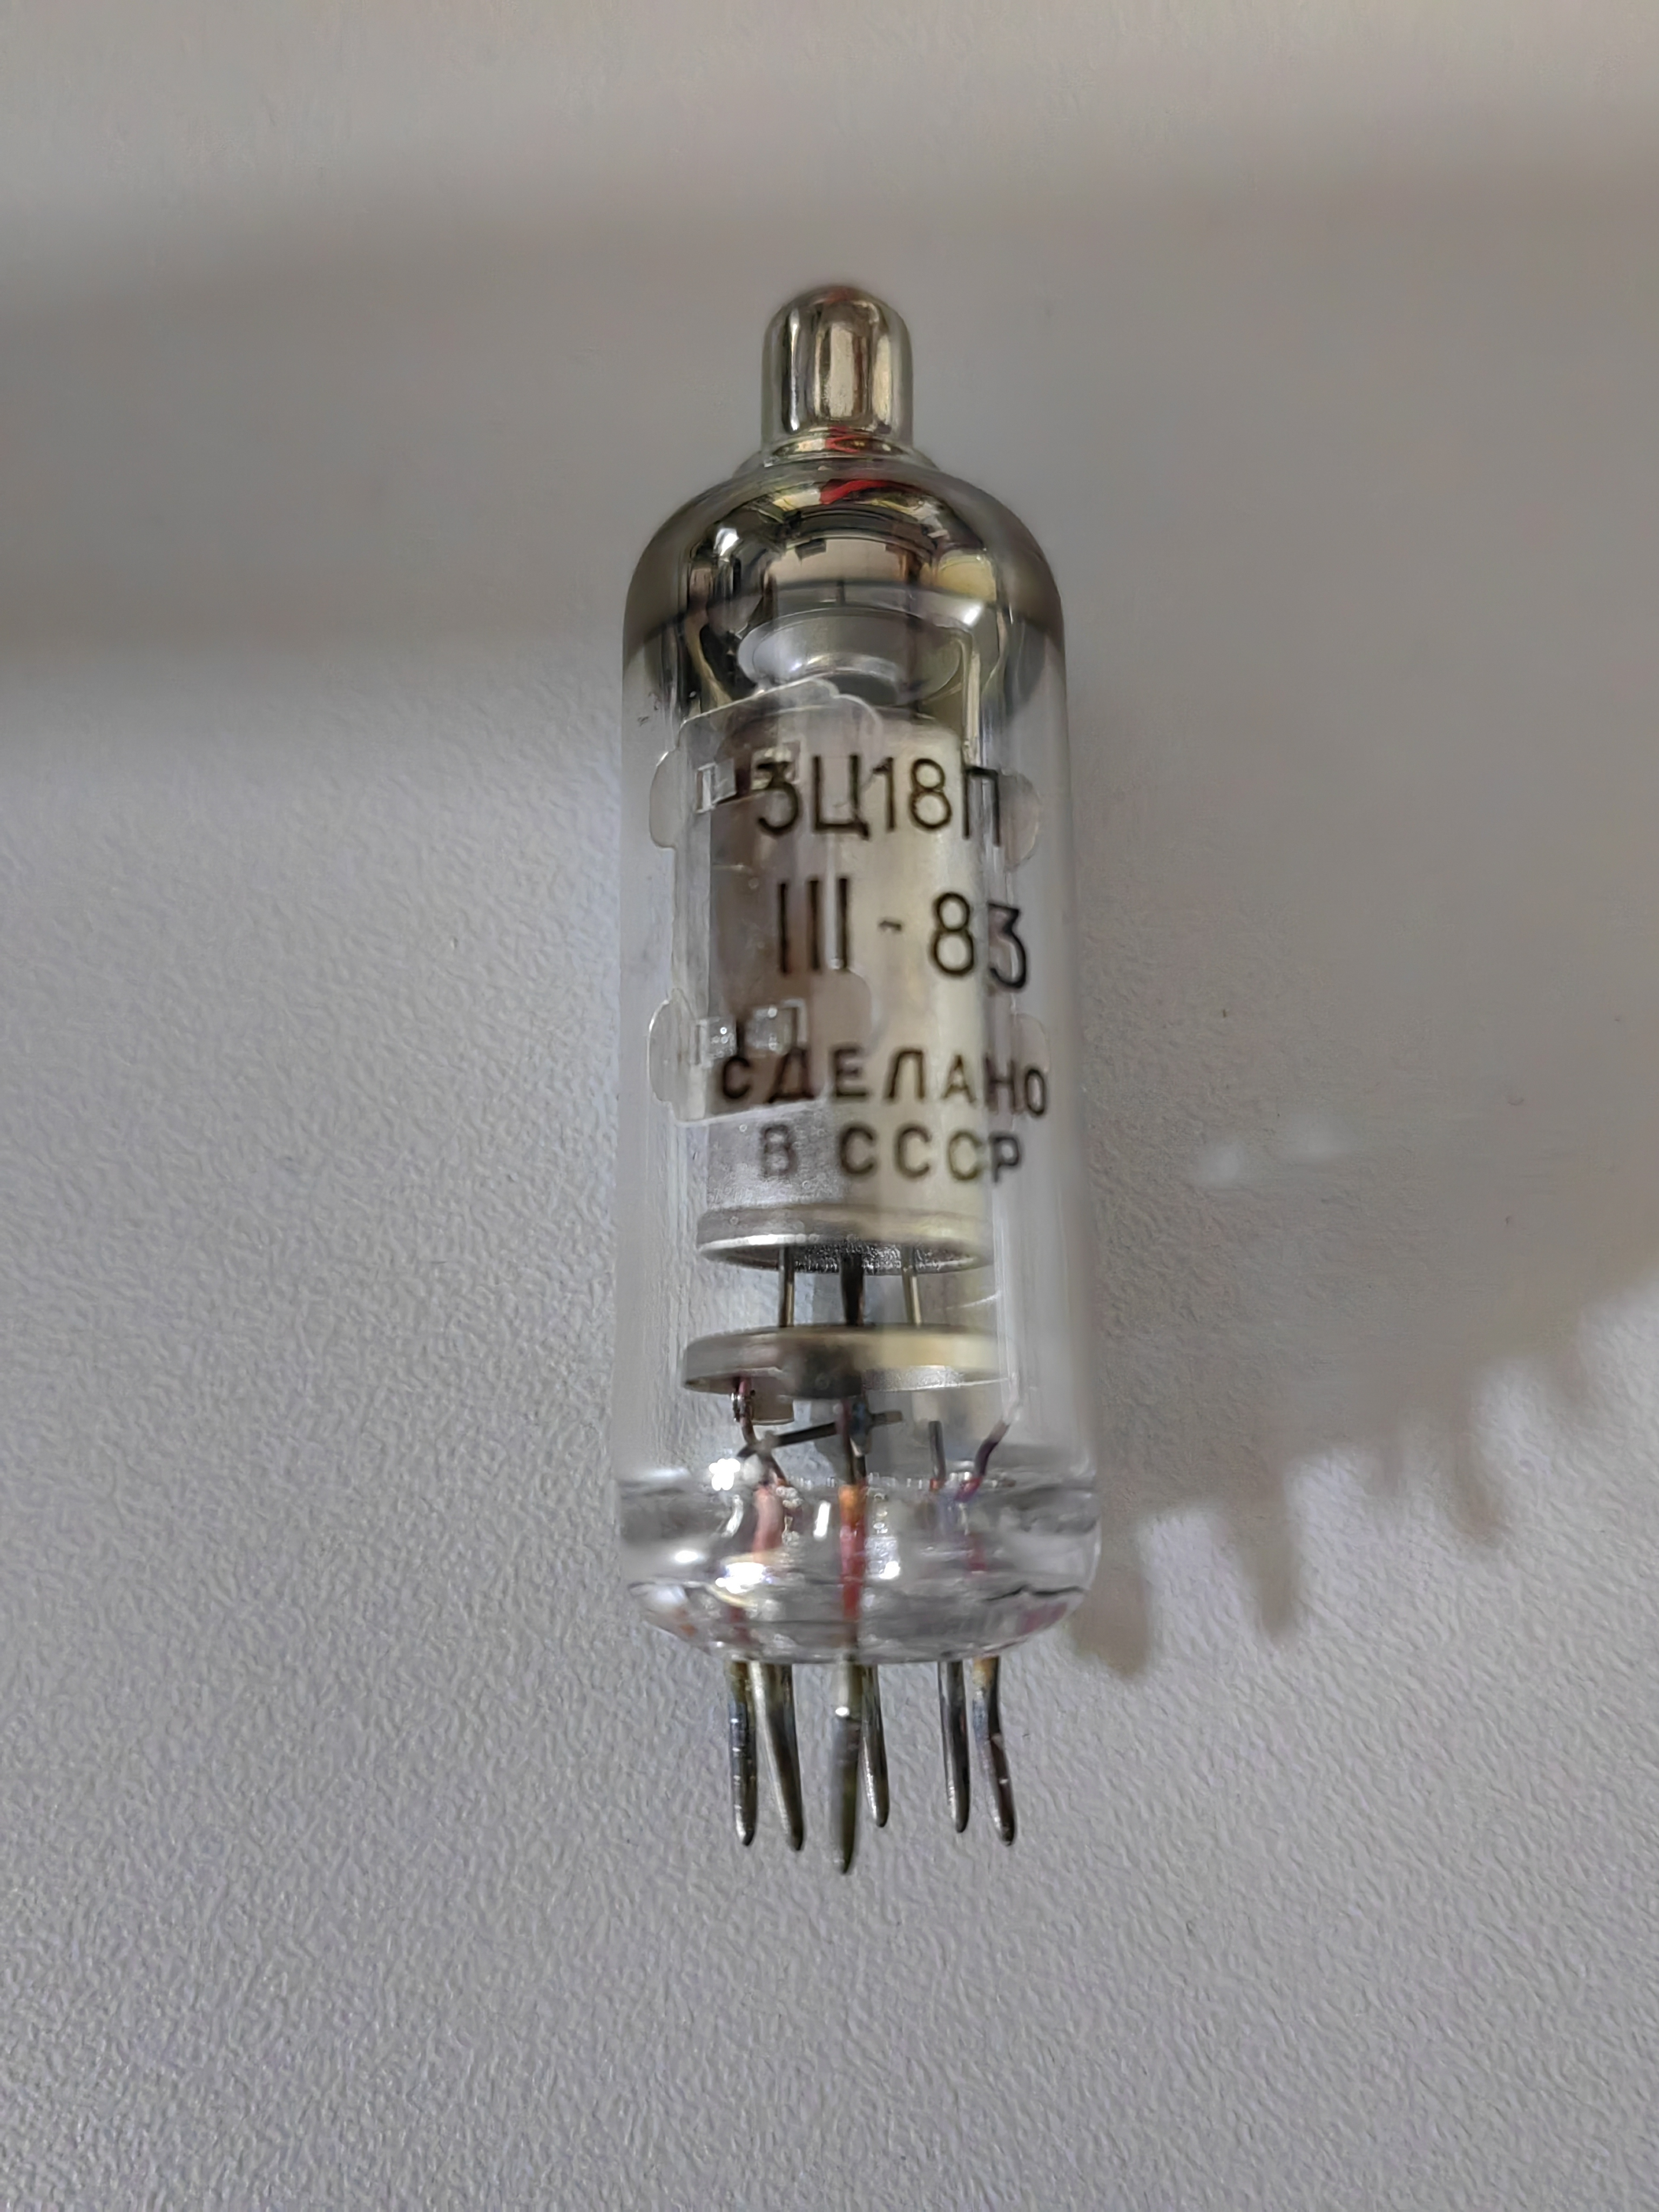
\includegraphics[scale=0.06]{./pics/diod.jpg}
     \captionof{figure}{Используемый диод}
\end{tabular}

\subsection{Определение температуры при помощи пиромера}



\begin{tabular}{m{0.45\linewidth}m{0.6\linewidth}}
При подачи напряжения на катод он начинал светиться. С Выставляя на пирометре температуру его собственной нити
можно было установить температуру катода
    &
     \centering
     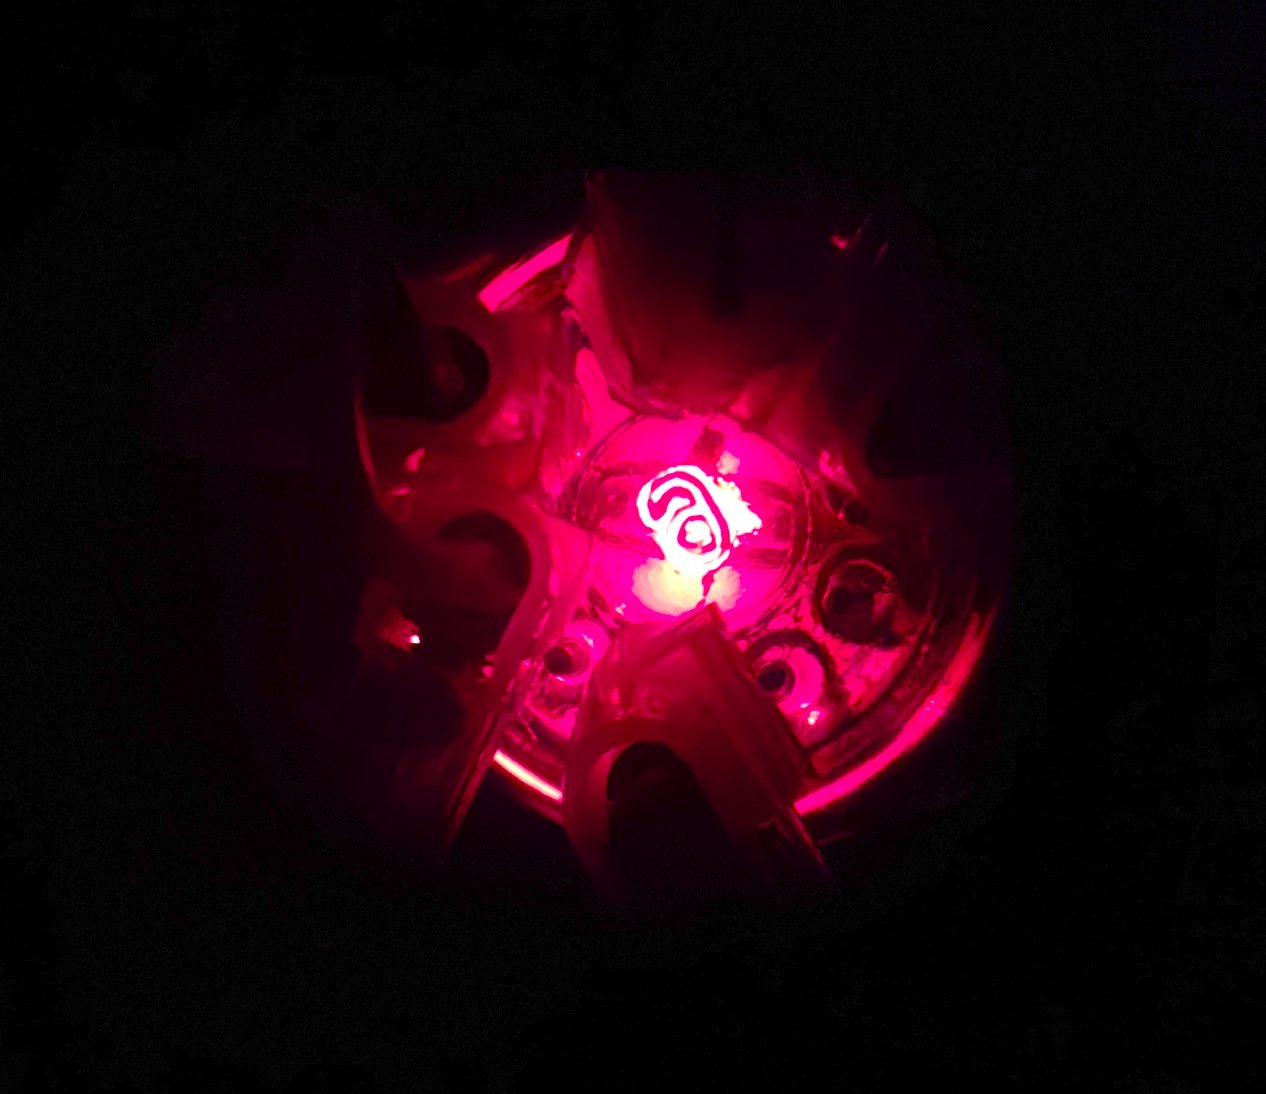
\includegraphics[scale=0.1]{./pics/red_katod.jpg}
     \captionof{figure}{Нагретый катод}
     \label{ris:temperature}
\end{tabular}

\begin{figure}[H]
        \centering

\end{figure}

\subsection{Определение температуры при помощи вольт-амперной характеристики}

В данном подходе снимается зависимость вольт-амперная характеристика для катода и определяется
зависимость зависимость и сопротивление. Далее пользовались следующем:

\begin{equation}
    R = R_0(1 + \alpha(T - T_0))
\end{equation}

\begin{equation}
    T = \frac{\frac{R}{R_0} - 1}{ \alpha} + T_0,
\end{equation}
где $\alpha$ - температурный коэффициент, который для вольфрама составляет
$$ \alpha = 5 * 10^{-3} \frac{1}{K} $$

\newpage

\section{Ход работы}

\begin{enumerate}
\item Сняли вольт-амперную характеристику катода, что помогло нам определить сопртивление
нити на линейном участке, по этим данным определили $R_0$.

\begin{figure}[H]
        \centering
        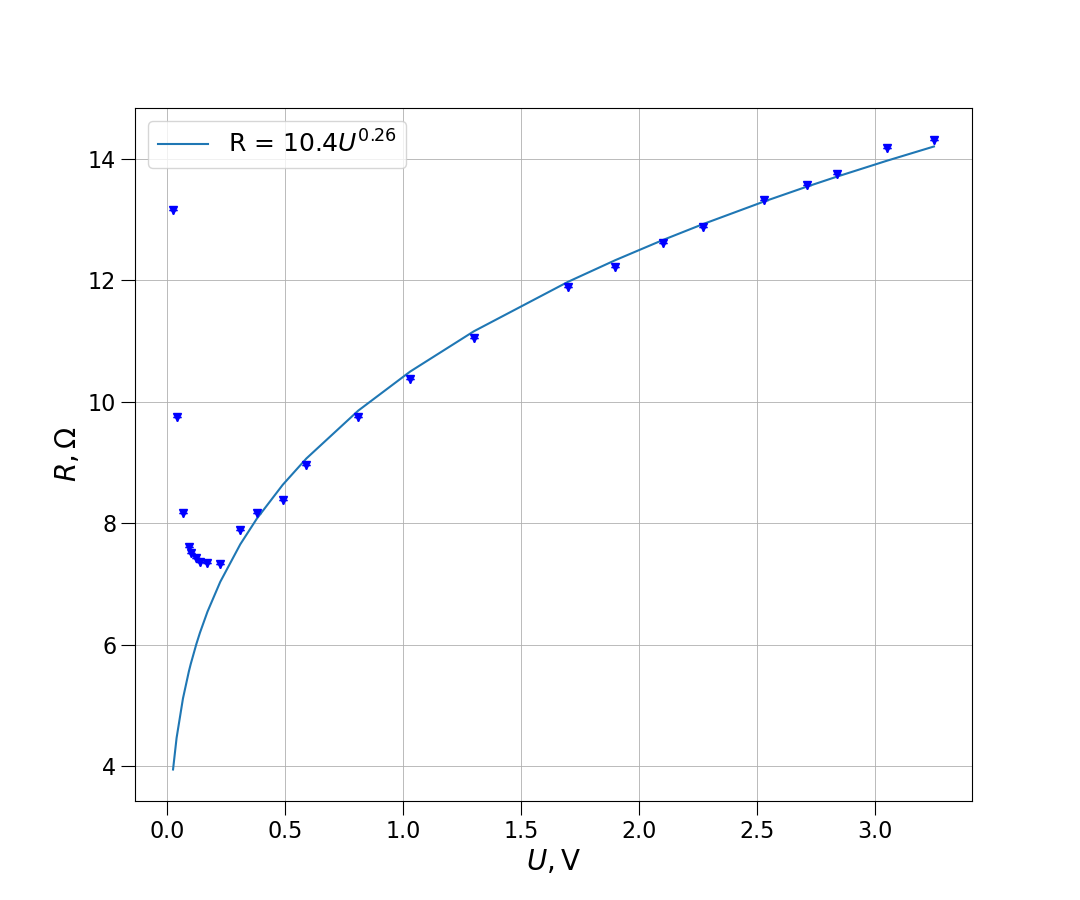
\includegraphics[scale=0.5]{./pics/resist.png}
        \caption{Зависимость сопротивления катода от напряжения}
        % \label{ris:setup_sh}
\end{figure}

% Для этого нашли наклон прямой аппроксимирующей линейный участок. $R_0 = (6.7 \pm 1) \; \text{Ом}$
% \begin{table}[H]
% 	\caption{$ y = ax + b $}
% 	\begin{center}
% 		\begin{tabular}{|c|c|c|}
% 			\hline
% 			& \text{Estimate} & \text{Standard Error} \\
% 			\hline
% 			a & 0.151 & 0,002 \\
% 			b & 0,0009 & $3*10^{-5}$ \\
% 			\hline
% 		\end{tabular}
% 	\end{center}
% \end{table}
% \newpage
\newpage
\item Выставляли на катоде в пределах $(2 - 3 \text{В}$) и по выходу на плато определяли
ток насыщения.

\begin{figure}[H]
        \centering
        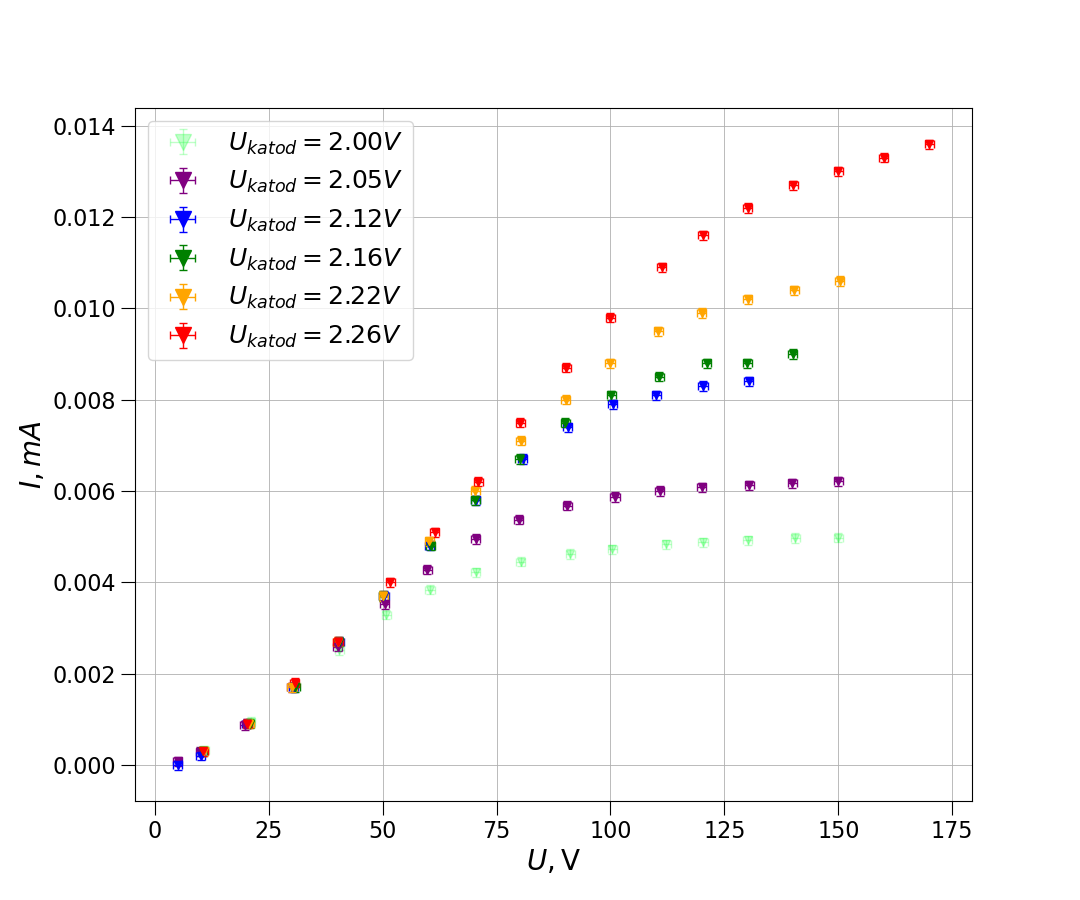
\includegraphics[scale=0.5]{./pics/different_plato.png}
        \caption{Зависимость тока от напряжения подаваемого на анод}
        % \label{ris:setup_sh}
\end{figure}

Получили следующие значения тока насыщения:

\begin{table}[!ht]
    \centering
    \begin{tabular}{|c|c|c|c|c|c|c|}
    \hline
        $U_{\text{накала}} \pm 0.01$, В      & $2.00 $ & $2.05 $ & $2.12 $ & $2.16 $ & $2.22 $ & $2.26 $ \\ \hline
        $I_{\text{насыщения}}\pm 0.1$, мкАм  & $5.0$ & $6.3$ & $8.5$ & $9.0$ & $10.7$ & $13.7$ \\ \hline
    \end{tabular}
\end{table}
\newpage
\item Получив, зависимость из предыдущего пунка для значения температуры от сопротивления
$$    T = \frac{\frac{R}{R_0} - 1}{ \alpha} + T_0$$. Построили график в логарифмическом масштабе для
проверки формулы Ричардсона-Дэшмана и определения работы выхода.

\begin{figure}[H]
        \centering
        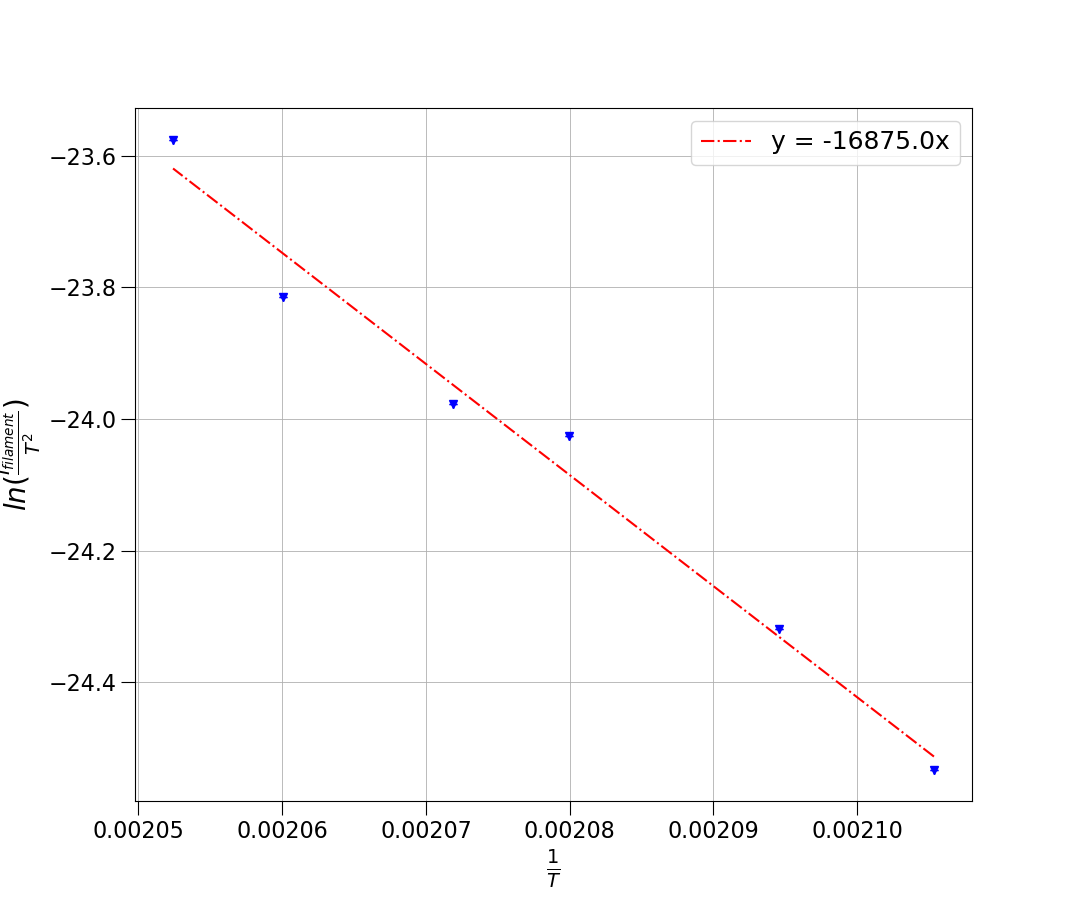
\includegraphics[scale=0.45]{./pics/richardson.png}
        \caption{График для проверки формулы Ричардсона-Дэшмана}
\end{figure}

\begin{table}[H]
	\caption{$ y = ax + b $}
	\begin{center}
		\begin{tabular}{|c|c|c|}
			\hline
			& \text{Estimate} & \text{Standard Error} \\
			\hline
			a & -16874 & 11 \\
			b & 952    & 1 \\
			\hline
		\end{tabular}
	\end{center}
\end{table}
Коэффициент корелляции $$R^2 = 0.98$$
\newpage


\newpage

\item По графику определили значения работы выхода для материала из которого сделана нить нашей лампы
$$W_o = k * tg(\phi)  = 1.4 \pm 0.1\; \text{эВ}$$,

Где $\phi$ - угол наклона прямой


\end{enumerate}

%-------------------------------------------------------------------------------------------

%-------------------------------------------------------------------------------------------


\section{Вывод}

В даннной работе проверялась зависимоть Ричардсона-Дэшмана для определения роботы выхода из катода
и были получены следующие результаты

$$W_o^{exp} = k * tg(\phi)  = 1.4 \pm 0.1\; \text{эВ}$$,
$$W_o^{th} = k * tg(\phi)  = 1.2 \; \text{эВ}$$,

\newpage

\section{P.S}

\begin{enumerate}
\item  В ходе работы несколько триодов были сожжены и получены из вольт-амперные характеристи
\begin{figure}[H]
        \centering
        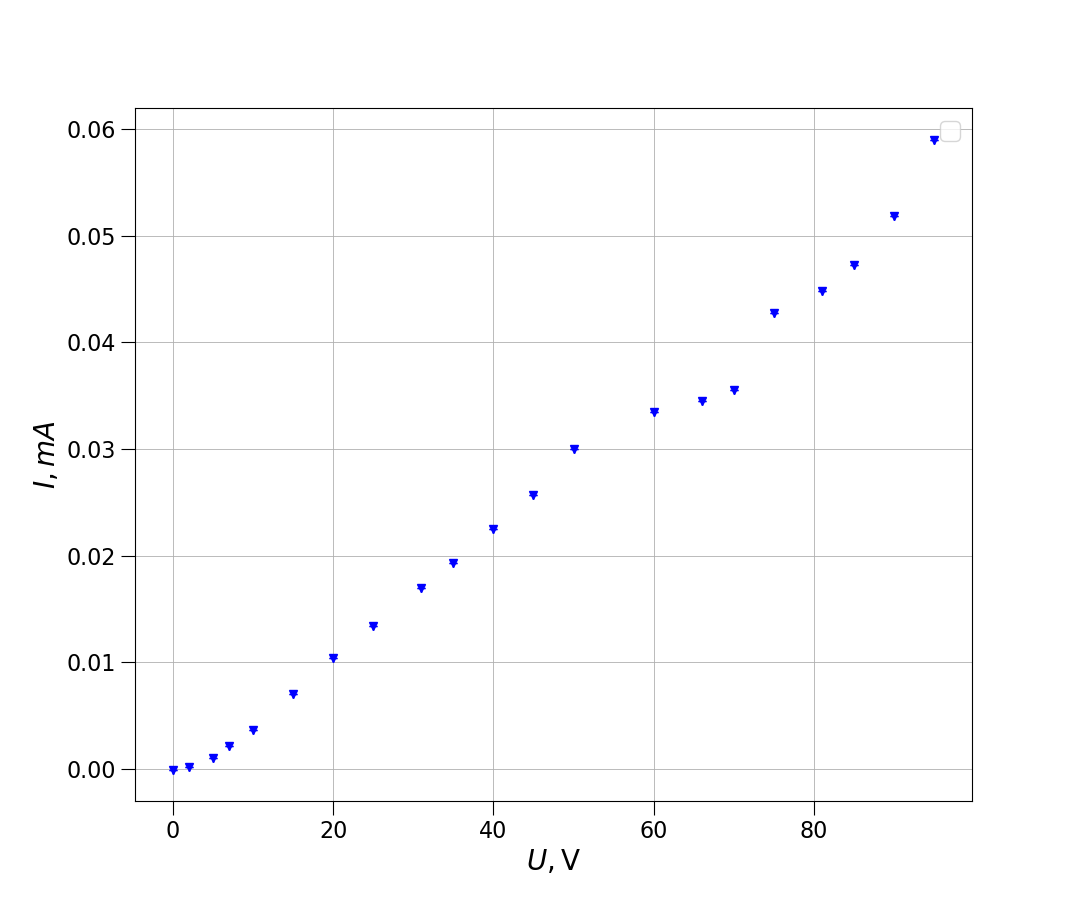
\includegraphics[scale=0.5]{./pics/failed_triod.png}
        \caption{Вольт-амперная характеристика переговревшего триода}
\end{figure}
\newpage

\item В работе также была определена зависимоть дифференциального сопротивления катода

\begin{figure}[H]
        \centering
        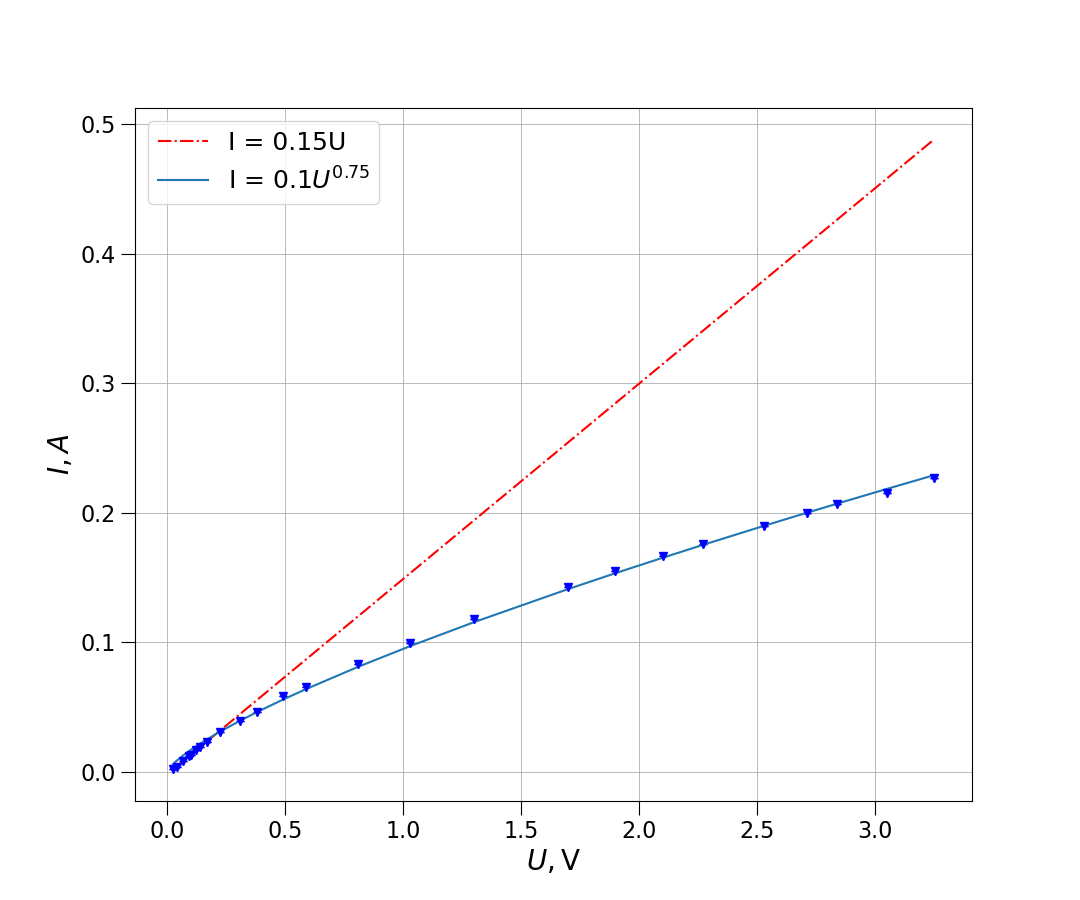
\includegraphics[scale=0.5]{./pics/diff_resist.png}
        \caption{Вольт-амперная характеристика катода}
        % \label{ris:setup_sh}
\end{figure}

Для этого нашли наклон прямой аппроксимирующей линейный участок. $R_0 = (6.7 \pm 1) \; \text{Ом}$
\begin{table}[H]
	\caption{$ y = ax + b $}
	\begin{center}
		\begin{tabular}{|c|c|c|}
			\hline
			& \text{Estimate} & \text{Standard Error} \\
			\hline
			a & 0.151 & 0,002 \\
			b & 0,0009 & $3*10^{-5}$ \\
			\hline
		\end{tabular}
	\end{center}
\end{table}

\newpage

\item Катод под напряжением...
\begin{figure}[H]
        \centering
        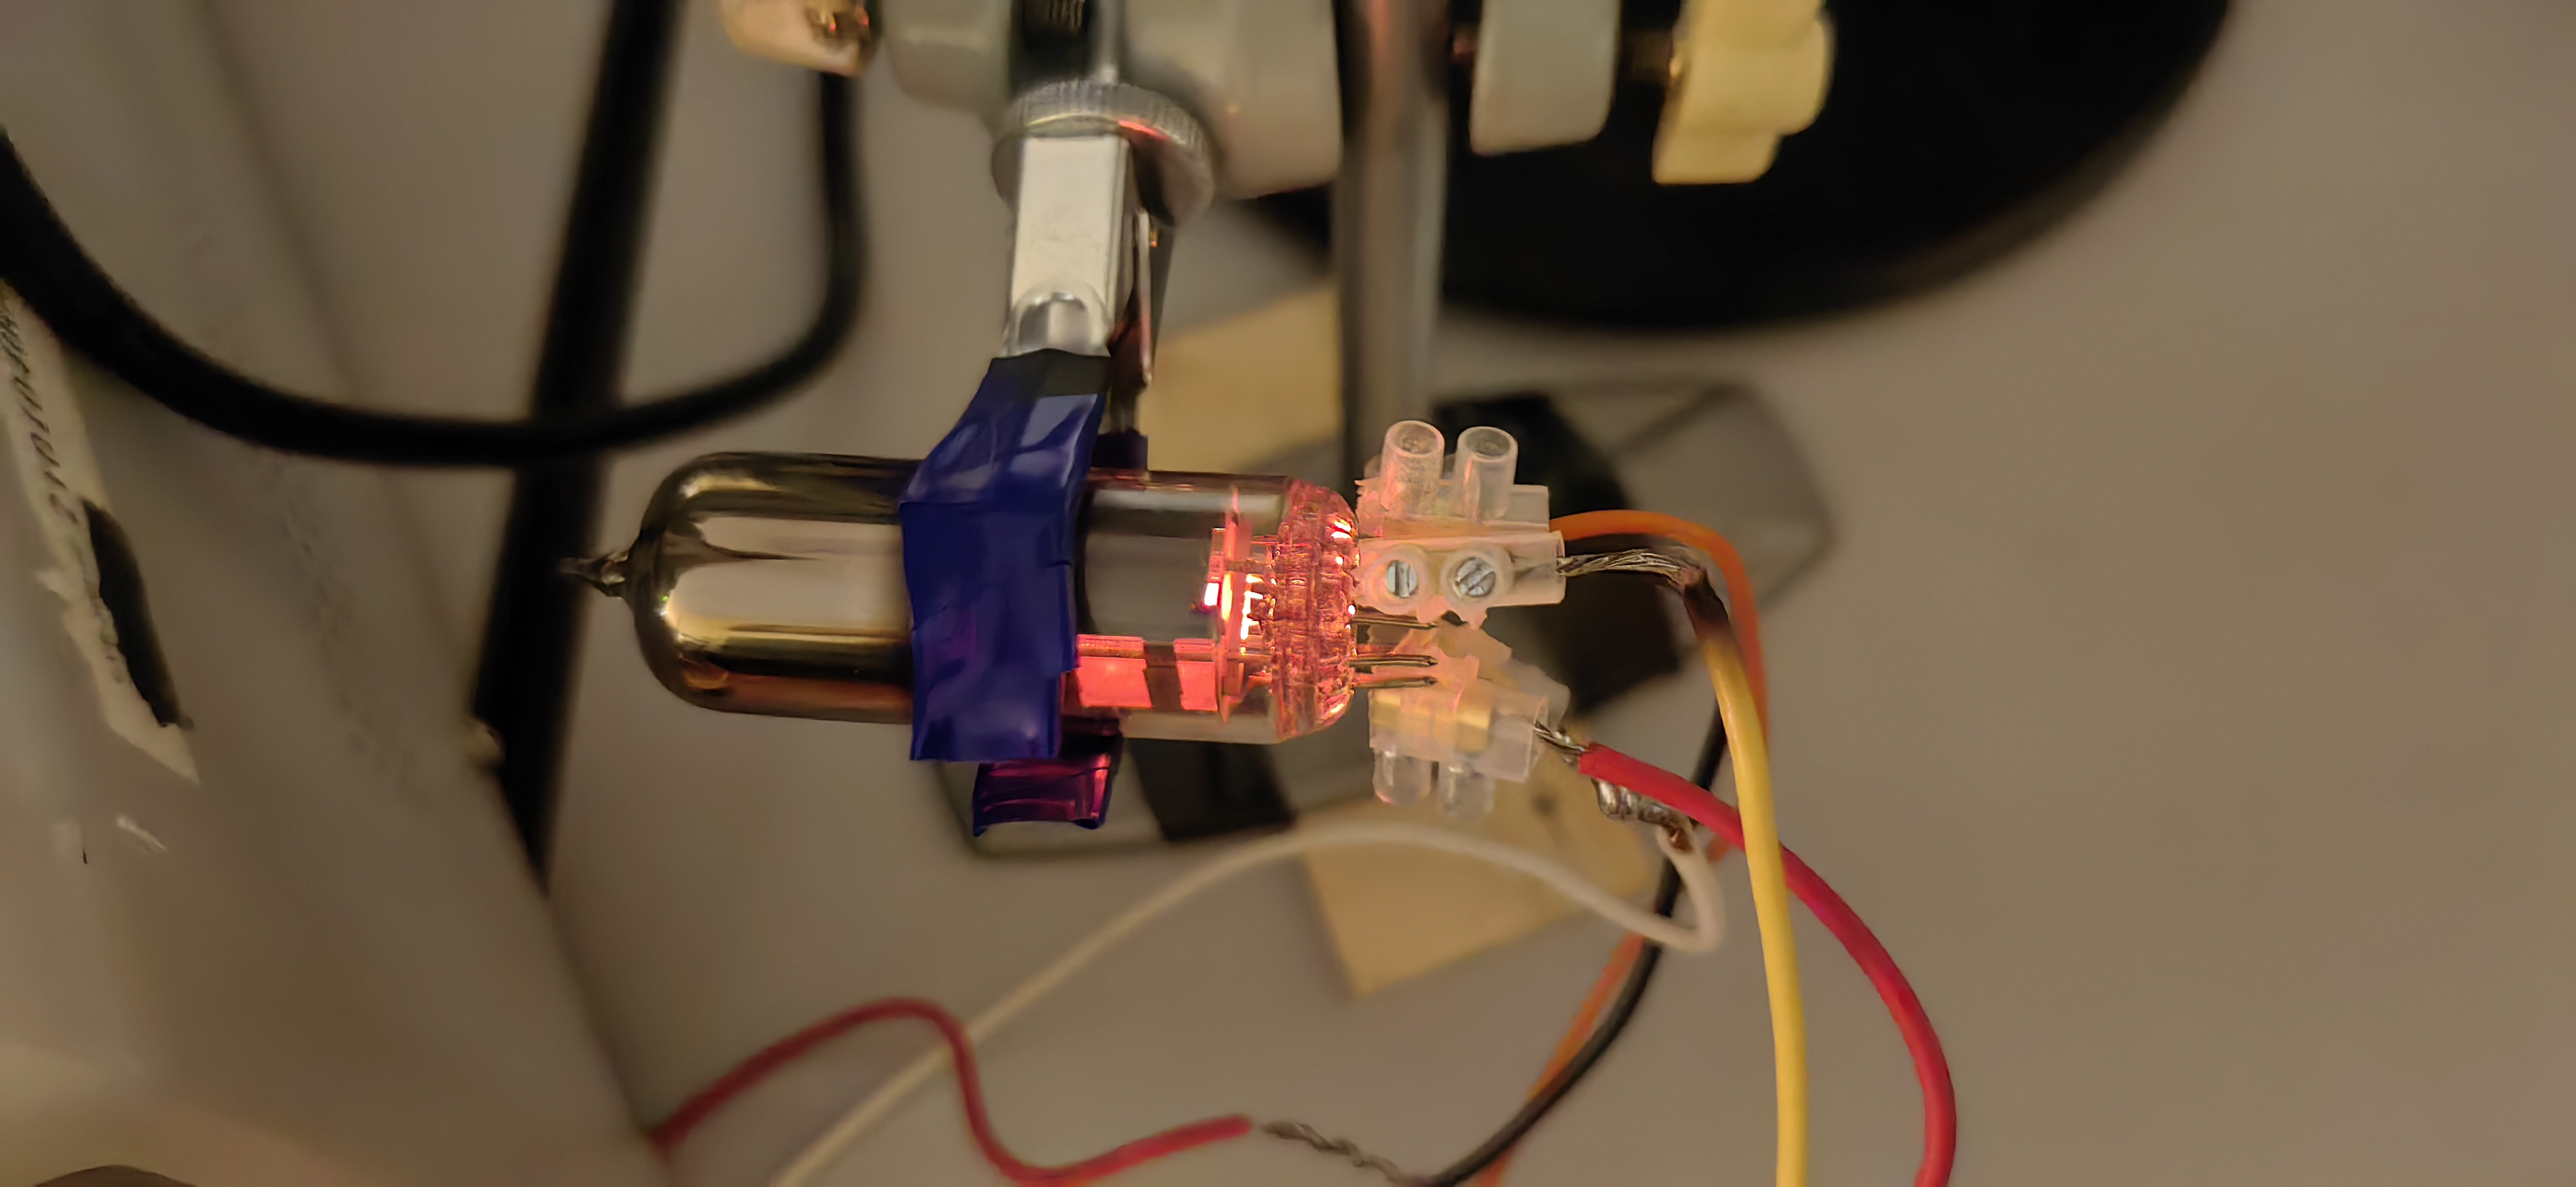
\includegraphics[scale=0.1]{./pics/shine_katod.jpg}
        \caption{Катод под напряжением...}
        % \label{ris:setup_sh}
\end{figure}

\newpage

\end{enumerate}



\end{document}




% \newpage
